\chapter{Convolutional Neural Network}
Convolutional Neural Networks (CNNs) are similar with the original of Neural Networks. It means that CNNs has also the score function and the loss function at the end of network. Neural Networks receive an input and pass it through a series of hidden layer but in CNNs is deeper. Each hidden layer is made from a set of neurons, where each neuron is full connected with all neurons of previous layer. The layers of the CNNs have neurons arranged in 3 dimensions: \textbf{width, height, depth}. CNNs transform the original image layer by layer from the original pixel value to the final class score. In CNNs, some layers contain the parameters but other don't. This chapter will describe the architecture and the detail of each layer in the CNNs.
\section{Architecture}
A CNN is made from the layers. The common layers in CNN are convolutional, nonlinear, pooling and full connected layers. CNN takes image as an input, pass it through the series of layers and get an ouput. Each layer has a difference function to transform the input to another layer. 
\begin{figure}[h]
	\centering
	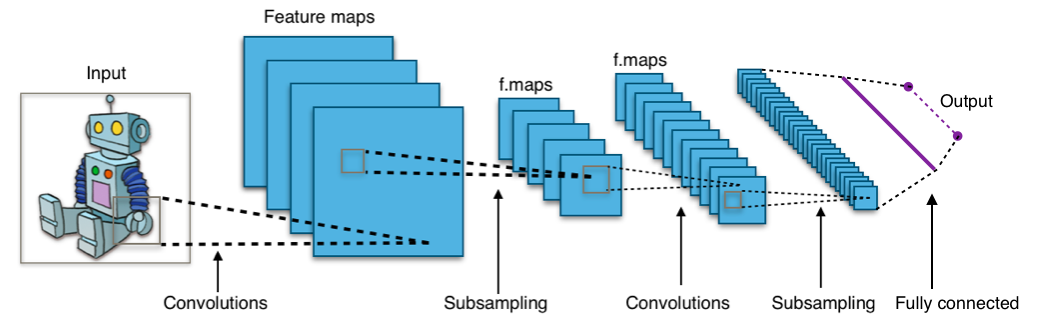
\includegraphics[scale=0.45]{images/cnn_architecture}
	\caption{An architecture of convolutional neural network}
	\label{figlncex}
\end{figure}~\\
\subsection{Convolutional layer}
Convolutional (CONV) layer computes a dot product between their weights and a small region in the input image for each small region in the input. At the output of neurons is combining the result  of the connected to local regions.\\[0.2cm]
CONV layer uses a set of learnable filters as parameters. Each filter is small spatially but extends the depth fo the input. During the forward pass, the filter is slided over each pixel of the input (from left to right, top to bottom) and calculate dot product between the entries of the filter and the input at this position. During the process, we can see the response of input for each filter such as the orientation of the edge or a blotch of some color on the firt layer. With an entire set of filters in each CONV layer, we will stack these activation maps along the depth dimension and procedure the output volume.\\[0.2cm]
Instead of connecting a neurons to all neurons in the previous layer, CONV connect each neurons to only a local region of the input. The spatial extent of this connectivity is a hyperparameter called the receptive field of the neuron (equal with the filter size). This extent has the depth axis is equal to the depth of the input. For example, if the input has size [32x32x3] and the filter size is [5x5] then each neuron in the CONV layer will have the weights to a [5x5x3] region in the input, and total of $5*5*3 = 75$ weights. This is the way that each neuron in CONV layer connected to the input; but how many neurons that we have in the output and how the order between the neurons. With 3 hyperparameters \textbf{depth, stride} and \textbf{zero-padding} will help us control the size of the CONV output.
\begin{itemize}
	\item \textbf{Depth}: corresponds to the number of filters we would like to use, each learning to look for something different in the input.
	\item \textbf{Stride}:  which we slide the filter. When the stride is 	1 then we move the filters one pixel at a time. If the stride is 2 (or more), then the filter will jump 2 (or more) at a time when we slide the filter.
	\item \textbf{Zero-padding}: pad the input with zeros arund the border.
\end{itemize}
\subsection{Pooling layer}
Pooling layer performs a downsampling operation along the spatial dimensions (width, height).
\subsection{Full connected layer}
Full connected layer computes the class scores of the input.
\section{Caffe framework}